\documentclass[a4paper, 10pt]{article}
\usepackage[T1]{fontenc}
\usepackage[utf8]{inputenc}
\usepackage[slovene]{babel}
\usepackage{csquotes}
\usepackage{lmodern}
\usepackage{amsmath}
\usepackage{leftidx}
%\usepackage[backend=biber, style=numeric]{biblatex}
\usepackage{amssymb}
\usepackage{amsthm}
\usepackage{amsfonts}
\usepackage{graphicx}
\usepackage{wrapfig}
\usepackage{amsthm}
\usepackage{mathrsfs}
\usepackage{mathtools}
\usepackage{url}
\usepackage{subfigure}
\usepackage{multirow}
\usepackage{lipsum}
\usepackage{wrapfig}
\usepackage{tikz}
\usepackage[format=plain, font=small, labelfont=bf, textfont=it, justification=centerlast]{caption}
\usepackage{booktabs}
\usepackage{siunitx}

\newtheorem{izr}{Izrek}
\newtheorem{posl}{Posledica}[izr]

\newcounter{defcount}
\newcounter{opombe}
\newcounter{primercount}

\newenvironment{opomba}{\begin{flushleft}\stepcounter{opombe}\textbf{Opomba \arabic{opombe}:}}{\hfill\end{flushleft}}
\setlength{\parindent}{0mm}

\newenvironment{primer}{\begin{flushleft}\stepcounter{zgledcount}\textbf{Primer \arabic{primercount}:}}{\hfill\end{flushleft}}
\setlength{\parindent}{0mm}

\newenvironment{definicija}{\begin{flushleft}\stepcounter{defcount}\textbf{Definicija \arabic{defcount}:}}{\hfill\end{flushleft}}
\setlength{\parindent}{0mm}

\newcommand{\naslov}[1]{\textit{#1}}
\newcommand{\abs}[1]{\ensuremath{\lvert #1 \rvert}}
\newcommand{\mth}[1]{\ensuremath{\mathbb{#1}}}
\newcommand{\R}{\mth{R}}
\newcommand{\Z}{\mth{Z}}
\newcommand{\Zp}{\mth{Z}^{+}}
\newcommand{\N}{\mth{N}}
\newcommand{\No}{\mth{N}_0}
\newcommand{\C}{\mth{C}}
\newcommand{\Qu}{\mth{Q}_u}
\newcommand{\pojem}[1]{\emph{#1}}
\newcommand{\con}{\ensuremath{\mathscr{C}}}
\newcommand{\padex}[2]{\ensuremath{{#1}^{\underline{#2}}}}
\newcommand{\rastx}[2]{\ensuremath{{#1}^{\bar{#2}}}}
\newcommand{\map}[3]{\ensuremath{{#1}: {#2} \rightarrow {#3}}}
\newcommand{\pra}[3]{{#1}{\ast}({#2}) = {#3}}

\title{Dinitzov algoritem \\ {\large Projektna naloga pri predmetu Osnove programiranja v diskretni matematiki}}
\date{3.~1.~2024}
\author{Jimmy Zakeršnik}
%===============================================================================
\begin{document}
	\maketitle
	\thispagestyle{empty}
	\newpage
	Sledeče definicije in opis algoritma so povzete po \cite{bib:even}.
	\begin{definicija}
		\begin{enumerate}
			\item Naj bo $G = (V, E)$ usmerjen povezan graf brez vzporednih povezav in brez povezav tipa $vv; v\in V$ ter $s, t\in V$ poljubni različni vozlišči na njem. Vozlišču $s$ pravimo \pojem{vir}, vozlišču $t$ pa \pojem{ponor}. Dodatno, naj bo $\map{c}{E}{\R^+}$ funkcija, ki vsaki povezavi priredi nenegativno realno število. Tej funkciji pravimo \pojem{kapaciteta}, peterici $N = (V, E, s, t, c)$ pa \pojem{omrežje}.
			\item Funkciji $\map{f}{E}{\R^+}$ pravimo \pojem{pretok}, če zadošča naslednjima pogojema: \begin{itemize}
				\item $\forall e\in E: 0 \leq f(e) \leq c(e)$
				\item $\forall v\in V \setminus \{s, t\}$: \[\sum_{\substack{u\in V \\ uv\in E}} f(uv) = \sum_{\substack{u\in V \\ vu\in E}} f(vu)\]
			\end{itemize}
			\item Količino $F = \sum_{\substack{u\in V \\ ut\in E}} f(ut) - \sum_{\substack{u\in V \\ tu\in E}} f(tu)$ imenujemo \pojem{skupni pretok} $f$ v omrežju $N$.
		\end{enumerate}
	\end{definicija}
	Mnogo problemov iz prakse (npr. sestavljanje prometnih omrežjih) lahko prevedemo na iskanje maksimalnega pretoka skozi neko omrežje. Eden izmed algoritmov, kako poiščemo maksimalni pretok, bo obravnavan v tej nalogi - Dinitzov Algoritem. Tukaj bo algoritem opisan, v priloženi datoteki \textit{Dinitz.py}, pa bo tudi implementiran.
	
	Dinitzov algoritem v prvi fazi iz danega omrežja $N = (V, E, s, t, c)$ in nekega začetnega pretoka $f$ sestavi t.~i.~ ">rezidualno omrežje"< $N' = (V, E', s, t, c')$, kjer je $E' = E \cup \{vu; uv\in E \land f(uv) > 0\}$in $c'(e) = \begin{cases}
		c(e) - f(e) &;~e\in E \\
		f(e) &;~e\in E'\setminus E
	\end{cases}$ t.~i.~">rezidualna kapaciteta"<. V drugi fazi algoritem s pomočjo $BFS$ algoritma sestavi t.~i.~ razslojeno omrežje $N'' = (V'', E'', s, t, c'')$ na naslednji način:
	\begin{enumerate}
		\item Poženi $BFS$ algoritem z vrhom v $s$. Če algoritem ne doseže ponorja $t$, je dan pretok $f$ že maksimalen.
		\item Če $BFS$ algoritem doseže $t$: $V'' = \bigcup_{i = 0}^{l} V_i$; $V_i$ so sloji, ki jih določi $BFS$ algoritem v $s$ in $V_l = \{t\}$.
		\item $E''_i = \{uv\in E'; u\in V_i \land v\in V_{i+1}\}$
		\item $E'' = \bigcup_{i = 0}^{l} E''_i$
		\item $c''$ je skrčitev $c'$ na $E''$
	\end{enumerate}
	V tretji fazi Dinitzov algoritem iz $f$ sestavi maksimalen pretok $f''$ v $N''$, ki ga tudi imenujemo zaporni pretok. To naredi tako, da v $N''$ poišče neko $(s, t)$-pot po povezavah (s pomočjo $DFS$ algoritma), ki še nimajo popolnoma zapolnjene kapacitete, in pretok $f''$ na tej poti poveča, kolikor lahko. To algoritem ponavlja, dokler lahko. Če pri iskanju poti algoritem zaide v ">slepo ulico"<, se vrne do vozlišča na katerem je bil, preden je zašel v njo in slepo ulico blokira, da vanjo ne zaide še enkrat.
	
	Na koncu se algoritem vrne v $N$ in pretok $f$ ">poveča"<: \[f(e) = \begin{cases}
		f(uv) + f''(uv)&;~ uv\in E \\
		f(uv) - f''(vu)&;~ vu \in E''\setminus E
	\end{cases}\] S tako popravljenim $f$ se algoritem vrne v prvo fazo. Ta cikel se ponavlja, dokler ne dobi pretoka $f$, ki je maksimalen.
	
	Za dano omrežje $N = (V, E, s, t, c)$ ima zgoraj opisani Dinitzov algoritem časovno zahtevnost $O(\abs{V}^2\abs{E})$. To časovno zahtevnost ima tudi implementiran algoritem DinitzAlg v \textit{Dinitz.py}, torej $O(\abs{V}^2\abs{E})$. Da je to res je treba preveriti samo, da je časovna zahtevnost vsakega koraka implementiranega algoritma enaka $O(\abs{V}\abs{E})$.
	Vidimo, da za sestavo stratificiranega omrežja $N''$ iz $N$ potrebujemo $O(\abs{E})$ in ker so vse ostale operacije v algoritmu, razen klic funkcije \textit{maksimalenpretok}, tudi opravljene v $O(\abs{E})$, bo časovna zahtevnost omenjene funkcije edino, kar bi lahko vplivalo na časovno zahtevnost koraka celega algoritma. Funkcija \textit{maksimalenpretok} pa ima časovno zahtevnost $O(\abs{V}\abs{E})$. Sledi torej, da ima ena izvedba zanke v funkciji \textit{DinitzAlg} časovno zahtevnost $O(\abs{V}\abs{E})$. Preostanek razmisleka sledi na enak način, kot je podan v viru \cite{bib:even}.
	
	V \textit{Dinitz.py} se koda izvede na treh testnih primerih: \textit{primer.txt}, \textit{primer2.txt} in \textit{primer3.txt}. Omenjena omrežja so narisana spodaj, skupaj z navedbo maksimalnega pretoka, kot ga izračuna \textit{DinitzAlg}.
	\begin{figure}[h!]
		\centering
		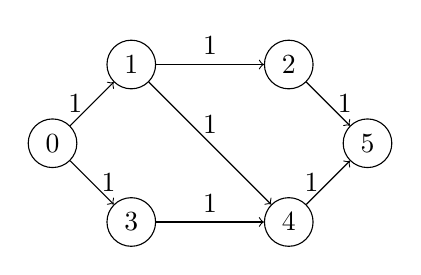
\begin{tikzpicture}
			\node[shape=circle,draw=black] (0) at (0,0) {0};
			\node[shape=circle,draw=black] (1) at (1,1) {1};
			\node[shape=circle,draw=black] (2) at (3,1) {2};
			\node[shape=circle,draw=black] (3) at (1,-1) {3};
			\node[shape=circle,draw=black] (4) at (3,-1) {4};
			\node[shape=circle,draw=black] (5) at (4,0) {5};
		
			\path [->] (0) edge node[left] {$1$} (1);
			\path [->] (0) edge node[right] {$1$} (3);
			\path [->] (1) edge node[above] {$1$} (2);
			\path [->] (1) edge node[above] {$1$} (4);
			\path [->] (2) edge node[right] {$1$} (5);
			\path [->] (3) edge node[above] {$1$} (4);
			\path [->] (4) edge node[left] {$1$} (5);
		\end{tikzpicture}
		\caption{Omrežje iz \textit{primer.txt} z maksimalnim pretokom $2$.}
	\end{figure}
	
	\begin{figure}[h!]
		\centering
		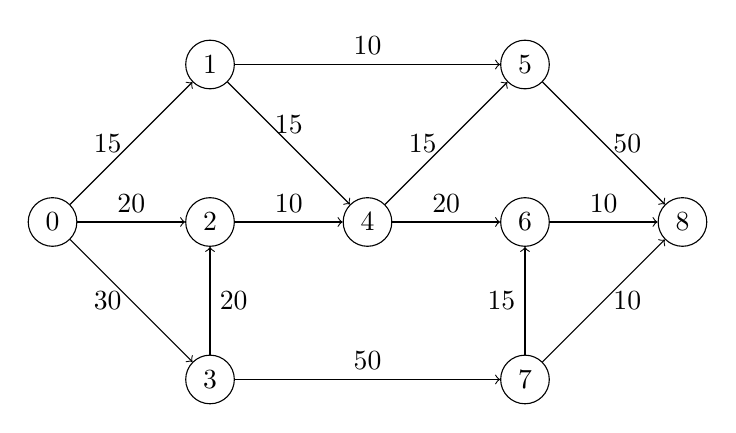
\begin{tikzpicture}
			\node[shape=circle,draw=black] (0) at (0,0) {0};
			\node[shape=circle,draw=black] (1) at (2,2) {1};
			\node[shape=circle,draw=black] (2) at (2,0) {2};
			\node[shape=circle,draw=black] (3) at (2,-2) {3};
			\node[shape=circle,draw=black] (4) at (4,0) {4};
			\node[shape=circle,draw=black] (5) at (6,2) {5};
			\node[shape=circle,draw=black] (6) at (6,0) {6};
			\node[shape=circle,draw=black] (7) at (6,-2) {7};
			\node[shape=circle,draw=black] (8) at (8,0) {8};
			
			\path [->] (0) edge node[left] {$15$} (1);
			\path [->] (0) edge node[above] {$20$} (2);
			\path [->] (0) edge node[left] {$30$} (3);
			\path [->] (1) edge node[above] {$15$} (4);
			\path [->] (1) edge node[above] {$10$} (5);
			\path [->] (2) edge node[above] {$10$} (4);
			\path [->] (3) edge node[right] {$20$} (2);
			\path [->] (3) edge node[above] {$50$} (7);
			\path [->] (4) edge node[left] {$15$} (5);
			\path [->] (4) edge node[above] {$20$} (6);
			\path [->] (5) edge node[right] {$50$} (8);
			\path [->] (6) edge node[above] {$10$} (8);
			\path [->] (7) edge node[left] {$15$} (6);
			\path [->] (7) edge node[right] {$10$} (8);
		\end{tikzpicture}
		\caption{Omrežje iz \textit{primer2.txt} z maksimalnim pretokom $45$.}
	\end{figure}
	
	\begin{figure}[h!]
		\centering
		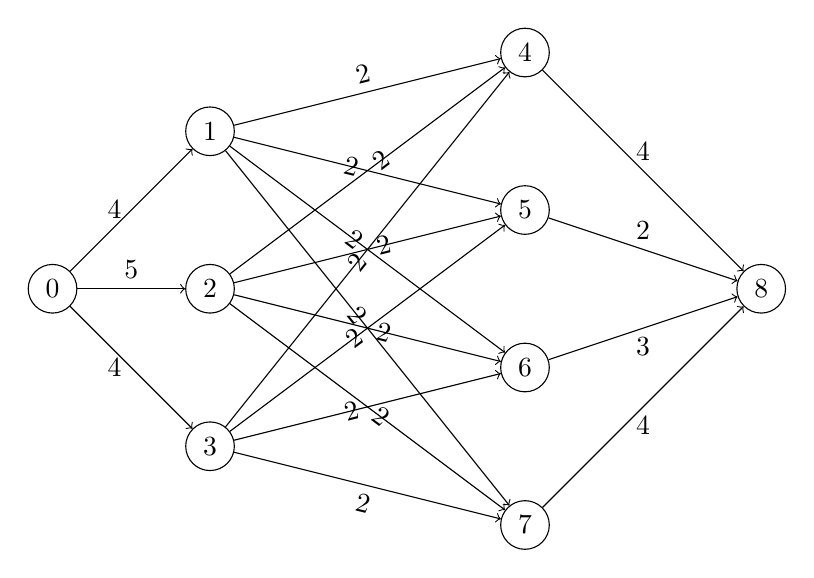
\begin{tikzpicture}
			\node[shape=circle,draw=black] (0) at (0,0) {0};
			\node[shape=circle,draw=black] (1) at (2,2) {1};
			\node[shape=circle,draw=black] (2) at (2,0) {2};
			\node[shape=circle,draw=black] (3) at (2,-2) {3};
			\node[shape=circle,draw=black] (4) at (6,3) {4};
			\node[shape=circle,draw=black] (5) at (6,1) {5};
			\node[shape=circle,draw=black] (6) at (6,-1) {6};
			\node[shape=circle,draw=black] (7) at (6,-3) {7};
			\node[shape=circle,draw=black] (8) at (9,0) {8};
			
			\path [->] (0) edge node[left] {$4$} (1);
			\path [->] (0) edge node[above] {$5$} (2);
			\path [->] (0) edge node[left] {$4$} (3);
			\path [->] (1) edge node[above, sloped] {$2$} (4);
			\path [->] (1) edge node[left, sloped] {$2$} (5);
			\path [->] (1) edge node[left, sloped] {$2$} (6);
			\path [->] (1) edge node[left, sloped] {$2$} (7);
			\path [->] (2) edge node[right, sloped] {$2$} (4);
			\path [->] (2) edge node[right, sloped] {$2$} (5);
			\path [->] (2) edge node[right, sloped] {$2$} (6);
			\path [->] (2) edge node[right, sloped] {$2$} (7);
			\path [->] (3) edge node[left, sloped] {$2$} (4);
			\path [->] (3) edge node[left, sloped] {$2$} (5);
			\path [->] (3) edge node[left, sloped] {$2$} (6);
			\path [->] (3) edge node[below, sloped] {$2$} (7);
			\path [->] (4) edge node[above] {$4$} (8);
			\path [->] (5) edge node[above] {$2$} (8);
			\path [->] (6) edge node[below] {$3$} (8);
			\path [->] (7) edge node[below] {$4$} (8);
		\end{tikzpicture}
		\caption{Omrežje iz \textit{primer3.txt} z maksimalnim pretokom $13$.}
	\end{figure}
	
\begin{thebibliography}{99}
	
	\bibitem{bib:even} S.~Even in G.~Even, \emph{Graph algorithms, 2nd edition}, Cambridge University Press, 2012, str.\ 85--102.
	
	\bibitem{bib:wiki} \emph{Dinic's algorithm}, v: Wikipedia, the free encyclopedia, [ogled 3.~1.~2024], dostopno na \url{https://en.wikipedia.org/wiki/Dinic%27s_algorithm}.
	
\end{thebibliography}
\end{document}